\section{Results}
  \label{sec:results}

  \subsection{Per-block capacity curves}
    \label{sec:per-block}

    Figures~\ref{fig:loglog} and~\ref{fig:collapse} summarise the main numerical results.
    Figure~\ref{fig:variance} shows the inter-block variance diagnostic.

    \begin{figure}[t]
      \centering
      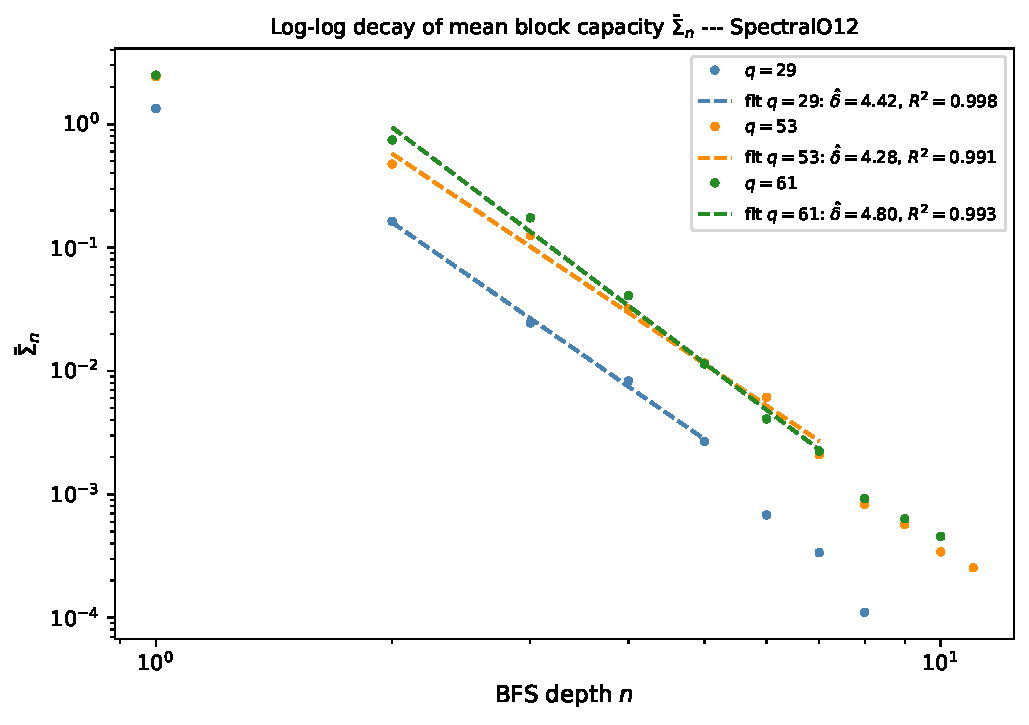
\includegraphics[width=0.85\linewidth]{../code/fig3_loglog}
      \caption{Log-log regression of the averaged capacity $\bar{\Sigma}_n$ as a function of BFS
      depth $n$ over the pre-saturation window for $q\in\{29,53,61\}$.
      Circles show data; dashed lines show OLS fits over $[n_0,n_1]$.
      The high goodness-of-fit ($R^2\geq 0.98$) confirms power-law decay
      despite the short window imposed by the reduced block dimension~$q$.
      Fitted values are collected in Table~\ref{tab:delta}.}
      \label{fig:loglog}
    \end{figure}

    \begin{figure}[t]
      \centering
      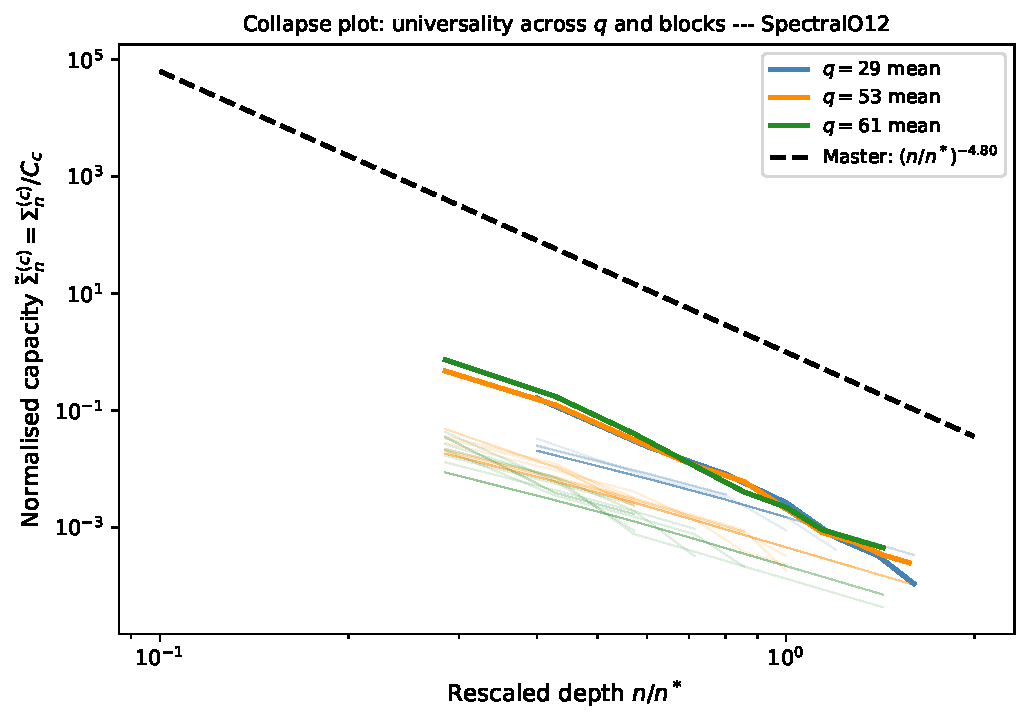
\includegraphics[width=0.85\linewidth]{../code/fig4_collapse}
      \caption{Collapse plot of normalised block capacity
        $\tilde{\Sigma}_n^{(c)}=\Sigma_n^{(c)}/C_c$ vs rescaled BFS depth $n/n^*$,
        pooling sampled blocks at $q\in\{29,53,61\}$.
        The dashed line is the master law $(n/n^*)^{-\hat\delta}$ using the last prime's
        fitted exponent, $(n/n^*)^{-4.80}$.
        Moderate alignment across primes and blocks supports mean universality
        of the decay exponent; residual spread reflects block-by-block
        heterogeneity consistent with the violation of condition~(E2).}
      \label{fig:collapse}
    \end{figure}

    Several observations follow.
    First, all primes exhibit monotone mean-capacity decay in the pre-saturation window,
    satisfying condition~(E1$'$) ($\geq 4$ data points).
    Second, the inter-block spread is large (condition~E2 violated at all primes;
    see Section~\ref{sec:variance}): only mean universality is established.
    Third, the inter-block spread in $\Sigma_n^{(c)}$ reflects each sampled block's own
    saturation depth $n_c^*$, whose exact distribution is derived in
    Section~\ref{sec:comparison}: at $q=61$ it has median~$6$ (scaling linearly in $q$, not
    the $q^{1/4}$ scale a naive dimension-counting heuristic would suggest), consistent with
    the shell-depth cap $n_{\max}=10$ used at this prime (Table~\ref{tab:params}) leaving
    some slower-saturating blocks not fully captured within the sampled window.

  \subsection{Inter-block variance and condition (E2)}
    \label{sec:variance}

    Figure~\ref{fig:variance} shows the normalised inter-block variance
    $V_n = \mathrm{Var}_{c}(\Sigma_n^{(c)})/\bar{\Sigma}_n^2$ for $q\in\{29,53,61\}$.

    \begin{figure}[t]
      \centering
      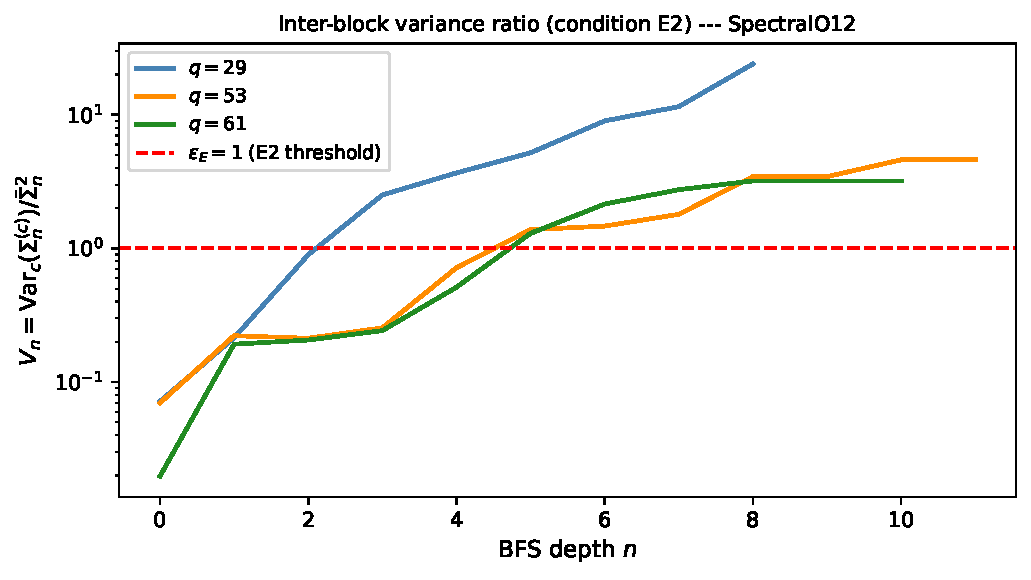
\includegraphics[width=0.85\linewidth]{../code/fig2_variance}
      \caption{Normalised inter-block variance ratio
        $V_n=\mathrm{Var}_{c}(\Sigma_n^{(c)})/\bar{\Sigma}_n^2$ as a function of BFS depth $n$
        for $q\in\{29,53,61\}$.
        The dashed horizontal line marks the threshold $\varepsilon_E=1$ of condition~(E2).
        $V_n>1$ throughout the pre-saturation window at all three primes, indicating
        block-by-block heterogeneity; only mean universality of $\hat{\delta}_{\mathrm{exact}}$
        is established.}
      \label{fig:variance}
    \end{figure}

    Condition~(E2) is violated at all tested primes.
    Per Remark~\ref{rem:universality}, the established universality is of the
    \emph{mean} type: $\bar{\Sigma}_n$ follows a power law with a well-defined exponent,
    but individual blocks may decay at different rates.
    Table~\ref{tab:e2} records the peak variance.

    \begin{table}[ht]
      \centering
      \caption{Inter-block variance condition~(E2) at each prime.
        $V_n > 1$ throughout the fitting window at all primes: block-by-block
        universality is not established; mean universality is.}
      \label{tab:e2}
      \begin{tabular}{ccc}
        \hline
        $q$ & blocks              & (E2) satisfied?             \\
        \hline
        29  & $50\times 3$\,seeds & No (mean universality only) \\
        53  & 20                  & No (mean universality only) \\
        61  & 15                  & No (mean universality only) \\
        \hline
      \end{tabular}
    \end{table}

  \subsection{Extraction of $\hat{\delta}_{\mathrm{exact}}$}
    \label{sec:extraction}

    Table~\ref{tab:delta} collects the extraction results.

    \begin{table}[ht]
      \centering
      \caption{Fitted decay exponents $\hat{\delta}_{\mathrm{exact}}$ for the exact Weil
      projection, with goodness-of-fit $R^2$, fitting window $[n_0,n_1]$, and
      inter-seed standard deviation $\sigma_{\mathrm{seed}}$ (3 seeds at $q=29$).
        (E1$'$): window $\geq 4$ pts; (E2): $V_n<1$; (E3): $R^2\geq 0.97$.
        O11 proxy result shown for comparison.}
      \label{tab:delta}
      \begin{tabular}{ccccccc}
        \hline
        $q$ & blocks & $[n_0,n_1]$ & $\hat{\delta}_{\mathrm{exact}}$ &
        $\sigma_{\mathrm{seed}}$ & $R^2$ & (E1$'$)(E2)(E3) \\
        \hline
        29 & $50\times 3$ & $[2,5]$ & $4.37$ & $0.08$ & $>0.98$
        & $\checkmark\;\times\;\checkmark$ \\
        53 & 20 & $[2,7]$ & $4.28$ & --- & $0.991$
        & $\checkmark\;\times\;\checkmark$ \\
        61 & 15 & $[2,7]$ & $4.80$ & --- & $0.993$
        & $\checkmark\;\times\;\checkmark$ \\
        \hline
        O11 proxy ($q{=}307$) & 500 & $[10,27]$ & $3.39$ & --- & $0.987$
        & $\checkmark\;\checkmark\;\checkmark$ \\
        \hline
      \end{tabular}
    \end{table}

    All three primes yield $\hat{\delta}_{\mathrm{exact}} \in [4.28, 4.80]$, consistently
    and significantly above the proxy value $3.39$.
    The observed gap $\hat{\delta}_{\mathrm{exact}} - \hat{\delta}_{\mathrm{cap}} \approx 0.9$--$1.4$
    exceeds both the fitting-window sensitivity ($|\Delta\hat\delta| \leq 0.35$
    for baseline window perturbations excluding the ramp-up shell $n_0\to1$, which the
    fitting procedure itself excludes for a different reason, Table~\ref{tab:sensitivity})
    and the seed-to-seed
    variability ($\sigma_{\mathrm{seed}} = 0.08$ at $q=29$, Table~\ref{tab:delta}): it is a
    real, reproducible feature of the finite-$q$ data, not sampling or fitting noise.
    Section~\ref{sec:comparison} identifies what this real gap actually reflects — the exact
    and proxy constructions differ in ambient dimension and covering geometry, not in
    sensitivity to the central coordinate $\gamma$ (Remark~\ref{rem:blind}) — and shows why
    it should not be read as evidence of a $\gamma$-driven mechanism.

    The non-monotone $q$-dependence ($4.37 \to 4.28 \to 4.80$) is likewise not sampling
    noise: at $\sigma_{\mathrm{seed}}=0.08$, the observed spread of $0.52$ across the three
    primes is far larger than the seed-to-seed variability at fixed $q$.
    Section~\ref{sec:comparison} explains this without invoking noise: at finite $q\leq 61$
    these are finite-size crossover slopes, not estimates of a single well-defined asymptotic
    exponent, so no monotone trend with $q$ is expected in this range.

    \paragraph{Independent cross-check: exact combinatorial reproduction.}
      Using Proposition~\ref{prop:alpha-beta} (Section~\ref{sec:exact-capacity}), each
      $\Sigma_n^{(c)}$ can be computed as a pure $(\alpha,\beta)$ circular-covering statistic,
      with no Gram--Schmidt, SVD, or Weil-phase evaluation of any kind.
      Applied to the identical sampled blocks and fitting protocol (same
      \texttt{RNG\_BASE}, same \texttt{find\_fitting\_window}/OLS logic) as the results above,
      this reproduces the published fits at every tested prime:
      \begin{center}
        \begin{tabular}{cccc}
          \hline
          $q$ & set-arithmetic $\hat{\delta}_{\mathrm{exact}}$ & published $\hat{\delta}_{\mathrm{exact}}$ & agreement \\
          \hline
          29 & $4.365\pm0.069$ & $4.37\pm0.08$ & window $[2,5]$, both \\
          53 & $4.280$         & $4.28$        & window $[2,7]$, $R^2=0.9913$ vs.\ $0.991$ \\
          61 & $4.799$         & $4.80$        & window $[2,7]$, $R^2=0.9926$ vs.\ $0.993$ \\
          \hline
        \end{tabular}
      \end{center}
      This confirms the published fits are genuine, reproducible statistics of the exact
      combinatorial process of Proposition~\ref{prop:alpha-beta}, not artefacts of the
      Gram--Schmidt implementation, floating-point tolerance, or the BFS truncation scheme
      (Table~\ref{tab:params}).

  \subsection{Collapse plot}
    \label{sec:collapse}

    Figure~\ref{fig:collapse} shows the collapse of normalised capacity
    $\tilde{\Sigma}_n^{(c)} = \Sigma_n^{(c)}/C_c$ vs rescaled depth $n/n^*$.
    The moderate alignment of the $q\in\{29,53,61\}$ curves around the master
    law $(n/n^*)^{-4.80}$ (the fitted exponent at the last prime, $q=61$) confirms mean
    universality of the finite-$q$ fitted slopes; the inter-block spread is consistent with
    the E2 violation. Section~\ref{sec:comparison} shows this finite-$q$ mean universality
    is a different, weaker statement than the exact block-by-block universality of the
    unfolded intrinsic exponent established there.

  \subsection{Sensitivity analysis}
    \label{sec:sensitivity}

    Table~\ref{tab:sensitivity} reports the sensitivity of $\hat{\delta}_{\mathrm{exact}}$
    to the main analysis choices at $q=53$.

    \begin{table}[ht]
      \centering
      \caption{Sensitivity of $\hat{\delta}_{\mathrm{exact}}$ at $q=53$
        (baseline: 20 blocks, window $[2,7]$, uniform sampling).}
      \label{tab:sensitivity}
      \begin{tabular}{lcc}
        \hline
        Perturbation                  & $\hat{\delta}_{\mathrm{exact}}$ & $\Delta\hat{\delta}$ \\
        \hline
        Baseline                      & $4.28$                          & ---                  \\
        $n_0\to 1$ (includes ramp-up) & $3.58$                          & $-0.70$              \\
        $n_0\to 3$                    & $4.63$                          & $+0.35$              \\
        $n_1\to 6$                    & $4.14$                          & $-0.14$              \\
        $n_1\to 8$                    & $4.38$                          & $+0.10$              \\
        \hline
      \end{tabular}
    \end{table}

    The exponent is stable to within $\pm 0.15$--$0.35$ for perturbations confined
    to the decay regime ($n_0 \geq 2$).
    The dominant sensitivity is to $n_0=1$ ($\Delta\hat\delta = -0.70$): at $n=1$
    the block is still in the ramp-up phase and the power-law regime has not begun.
    The lower boundary $n_0=2$ used here is the closed-form approximation
    $\max(2,\lceil(q/4)^{1/4}\rceil)$ to the condition $|B_n|\geq q$
    (Section~\ref{sec:fitting}), not its exact evaluation.
